\chapter{Sekvenovanie DNA}

\label{kap:sekvenovanie}

Genetická informácia je v prírode často kódovaná deoxyribonukleovou kyselinou (DNA\footnote{z anglického 
\emph{\textbf{d}eoxyribo\textbf{n}ucleic \textbf{a}cid}}). DNA je tvorená dvoma vláknami spletenými
do tvaru dvojzávitnice. Každé vlákno obsahuje postupnosť dusíkatých báz, ktorá kóduje informáciu. V DNA 
sa 
vyskytujú štyri
dusíkaté bázy: adenín (\texttt{A}), cytozín (\texttt{C}), guanín (\texttt{G}) a tymín (\texttt{T}). Postupnosti báz v jednotlivých vláknach 
sú 
komplementárne: na pozíciách, kde má prvé vlákno adenín 
(resp. cytozín, guanín, tymín) má druhé vlákno tymín (resp. guanín, cytozín, adenín). Na 
zrekonštruovanie 
celej informácie nám teda stačí poznať poradie báz v jednom z vlákien.

Proces zisťovania poradia báz v DNA sa nazýva \emph{sekvenovanie} DNA. Techniky sekvenovania DNA
boli známe už v sedemdesiatych rokoch minulého storočia a od vtedy sa stále vyvíjajú. Pri sekvenovaní
sa určí poradie dusíkatých báz vo fragmentoch DNA, nazývaných \emph{čítania}. Z dostatočného počtu 
prekrývajúcich sa čítaní sa potom dá zrekonštruovať celá postupnosť báz v DNA. Pre rôzne sekvenačné 
technológie sú typické rôzne dĺžky čítaní, ktoré produkujú.

\section{Nanopórové sekvenovanie DNA}

Jednou z najnovších sekvenačných technológií je nanopórové sekvenovanie. Vyznačuje sa dlhými čítaniami,
nízkou cenou a dostupnosťou prvých dát už počas sekvenovania, ale aj veľkým množstvom chýb v 
jednotlivých čítaniach \cite{Laver2015}. Pri nanopórovom sekvenovaní sa vo vhodne zvolenej membráne vytvorí 
\emph{nanopór}, t. j. otvor s priemerom rádovo $1 \si{nm}$. Membránou sa oddelia dve komory s 
elektrolytom, pričom v jednej z komôr sa nachádza aj predpripravená vzorka DNA.
Po zavedení elektrického napätia medzi komorami začne nanopórom tiecť iónový prúd. Jedno vlákno DNA
 sa postupne oddeľuje od druhého a prechádza nanopórom (Obr. \ref{fig:nanopor}). Časť vlákna, 
ktorá sa práve nachádza v najužšej časti nanopóru, má vplyv na elektrický prúd tečúci cez nanopór. Rôzne 
bázy ovplyvňujú elektrický prúd rôznym spôsobom. Pri sekvenovaní sa meria priebeh elektrického prúdu v 
čase a na základe jeho zmien sa potom určuje, aké bázy prešli cez nanopór \cite{Branton2008}.

\begin{figure}[t]
\centerline{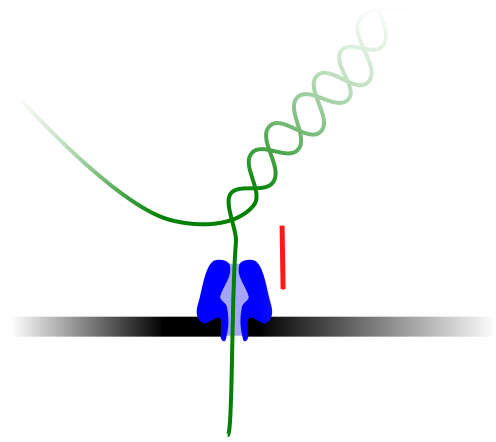
\includegraphics[width=0.7\textwidth]{images/nanopor}}
\caption{Prechod jedného vlákna DNA nanopórom.}
\label{fig:nanopor}
\end{figure}

V našej práci budeme pracovať s dátami zo sekvenátora MinION.
Prístroj MinION je nanopórový sekvenátor vyrábaný firmou Oxford Nanopore Technologies.
V sekvenátori MinION sa používa polymérová membrána, do ktorej sú 
zasadené proteínové nanopóry. Sekvenátor obsahuje stovky nanopórov, dokáže teda sekvenovať niekoľko DNA 
vlákien súčasne.
Vo verzii, s ktorou pracujeme, prechádza vlákno DNA cez nanopór rýchlosťou približne $400$ báz za 
sekundu. Hodnota elektrického prúdu sa zaznamenáva $4000$-krát za sekundu, teda v priemere zhruba $10$-
krát na bázu. Namerané hodnoty prúdu sa pre každé čítanie ukladajú do zvlášť súboru vo formáte 
\texttt{.fast5}. Tieto nespracované dáta budeme nazývať \emph{surový signál}.

\subsection{Normalizácia signálu}

Surový signál závisí nielen od úseku DNA nachádzajúceho sa v nanopóre, ale aj od ďalších faktorov, ktoré 
sa pre rôzne čítania môžu líšiť. Pred ďalším spracovaním je preto potrebné surový signál znormalizovať.

Jednou z metód normalizácie je \emph{mediánová normalizácia}, ktorú navrhujú Stoiber et. al. \cite{Stoiber2017}

\begin{definicia}
Nech $a_1, a_2, \dots, a_n \in \mathbb{R}$. Symbolom
$$\median{i=1}{n}(a_i)$$
budeme značiť medián hodnôt $a_1, a_2, \dots, a_n$.
\end{definicia}

\begin{definicia}
Nech $r_1, r_2, \dots, r_n$ sú namerané hodnoty surového signálu. Nech
 $$M = \median{i=1}{n}(r_i)$$ a nech $$D = \median{i=1}{n}(\abs*{r_i - M}) \text{.}$$

\emph{Mediánovo znormalizovaný} signál je postupnosť $s_1, s_2, \dots, s_n$ určená predpisom

$$s_i = \frac{r_i - M}{D} \text{.}$$

\end{definicia}

\subsection{Určovanie báz}

Na základe signálu nameraného zariadením MinION sa určuje, aké dusíkaté bázy prechádzali nanopórom, keď bol
tento signál zaznamenaný. Táto úloha je pomerne náročná a v súčasnosti sa stále vyvíjajú lepšie a
lepšie riešenia. Programy, ktoré určujú bázy, nazývame \emph{prekladače báz}.

Pri určovaní báz sa využíva fakt, že rôzne bázy pri svojom prechode nanopórom ovplyvňujú signál
rôznym charakteristickým spôsobom. V praxi však signál nie je ovplyvnený iba jednou bázou. Pracuje
sa preto s predpokladom, že signál je ovplyvnený $k$ po sebe idúcimi bázami, ktoré sú práve najbližšie
k nanopóru. Skupinám $k$ po sebe idúcich báz sa hovorí \emph{\kmer{y}}.

Ďalším problémom je, že vlákno DNA cez nanopór neprechádza konštantnou rýchlosťou. Jednotlivým bázam vo 
výslednej postupnosti preto môžu zodpovedať rôzne dlhé úseky signálu. Prvým krokom pri určovaní báz 
preto často býva rozdelenie signálu na úseky, v rámci ktorých bola hodnota signálu približne konštantná.
Týmto úsekom sa hovorí \emph{udalosti}. Pri ďalšom spracovaní sa predpokladá, že medzi jednotlivými 
udalosťami sa vlákno DNA väčšinou posunie o jednu bázu. Keďže však rozdelenie signálu na udalosti nemusí
presne zodpovedať posunom DNA vlákna v nanopóre, uvažuje sa aj možnosť, že sa vlákno medzi udalosťami 
neposunulo, prípadne posunulo o viac než jednu bázu.

Niektoré prekladače báz (napr. Nanocall \cite{Nanocall2017}) modelujú prechod DNA vlákna nanopórom ako 
skrytý Markovovský model. Na základe tohto
modelu sa Viterbiho algoritmom vypočíta najpravdepodobnejšia postupnosť báz, ktorá mohla vygenerovať 
pozorovaný signál.

Iné prekladače báz sú založené na rekurentných neurónových sieťach. Niektoré (napr. DeepNano 
\cite{DeepNano2017}) pracujú so signálom rozdeleným na udalosti, iné pracujú s nerozdeleným signálom 
(napr. Chiron \cite{Chiron2017}).

Najlepšie súčasné prekladače báz majú pre jedno čítanie presnosť okolo $85\%$ až $90\%$. Ak sa osekvenuje viac kópií rovnakej DNA, skombinovaním dostatočného počtu prekrývajúcich sa čítaní sa dá dosiahnuť presnosť okolo $99,9\%$ \cite{BasecallerComparison}.
